\documentclass[aspectratio=43]{beamer}

%\documentclass[handout]{beamer}
%% To make 4 per page
%\usepackage{pgfpages}
%\mode<handout>{\setbeamercolor{background canvas}{bg=white}}
%\pgfpagesuselayout{4 on 1}[letterpaper,landscape]%,border shrink=5mm]

\usetheme{default}
\usepackage{bm}
\usepackage{colortbl}

\usepackage{amsmath,amssymb,amsthm}
%\usepackage{subfigure}


% Fields and the like
\def\IC{\mathbb{C}}
\def\IF{\mathbb{F}}
\def\II{\mathbb{I}}
\def\IM{\mathbb{M}}
\def\IN{\mathbb{N}}
\def\IP{\mathbb{P}}
\def\IR{\mathbb{R}}
\def\IZ{\mathbb{Z}}

% Bold lowercase
\def\ba{\mathbf{a}}
\def\bb{\mathbf{b}}
\def\bc{\mathbf{c}}
\def\bd{\mathbf{d}}
\def\be{\mathbf{e}}
\def\bf{\mathbf{f}}
\def\bh{\mathbf{h}}
\def\bi{\mathbf{i}}
\def\bj{\mathbf{j}}
\def\bk{\mathbf{k}}
\def\bn{\mathbf{n}}
\def\bp{\mathbf{p}}
\def\br{\mathbf{r}}
\def\bs{\mathbf{s}}
\def\bu{\mathbf{u}}
\def\bv{\mathbf{v}}
\def\bw{\mathbf{w}}
\def\bx{\mathbf{x}}
\def\by{\mathbf{y}}
\def\bz{\mathbf{z}}

% Bold capitals
\def\bB{\mathbf{B}}
\def\bD{\mathbf{D}}
\def\bF{\mathbf{F}}
\def\bG{\mathbf{G}}
\def\bI{\mathbf{I}}
\def\bL{\mathbf{L}}
\def\bN{\mathbf{N}}
\def\bR{\mathbf{R}}
\def\bS{\mathbf{S}}
\def\bT{\mathbf{T}}
\def\bX{\mathbf{X}}

% Bold numbers
\def\b0{\mathbf{0}}

% Bold greek
\bmdefine{\bmu}{\bm{\mu}}
\def\bphi{\bm{\phi}}
\def\bvarphi{\bm{\varphi}}

% Bold red sentence
\def\boldred#1{{\color{red}\textbf{#1}}}
\def\defword#1{{\color{orange}\textbf{#1}}}

% Caligraphic letters
\def\A{\mathcal{A}}
\def\B{\mathcal{B}}
\def\C{\mathcal{C}}
\def\D{\mathcal{D}}
\def\E{\mathcal{E}}
\def\F{\mathcal{F}}
\def\G{\mathcal{G}}
\def\I{\mathcal{I}}
\def\L{\mathcal{L}}
\def\M{\mathcal{M}}
\def\P{\mathcal{P}}
\def\R{\mathcal{R}}
\def\S{\mathcal{S}}
\def\T{\mathcal{T}}
\def\U{\mathcal{U}}
\def\V{\mathcal{V}}

% tt font for code
\def\code#1{{\tt #1}}

% Operators and special symbols
\def\nbOne{{\mathchoice {\rm 1\mskip-4mu l} {\rm 1\mskip-4mu l}
{\rm 1\mskip-4.5mu l} {\rm 1\mskip-5mu l}}}
\def\cov{\ensuremath{\mathsf{cov}}}
\def\Var{\ensuremath{\mathsf{Var}\ }}
\def\Im{\textrm{Im}\;}
\def\Re{\textrm{Re}\;}
\def\det{\ensuremath{\mathsf{det}}}
\def\diag{\ensuremath{\mathsf{diag}}}
\def\nullspace{\ensuremath{\mathsf{null}}}
\def\nullity{\ensuremath{\mathsf{nullity}}}
\def\rank{\ensuremath{\mathsf{rank}}}
\def\range{\ensuremath{\mathsf{range}}}
\def\sgn{\ensuremath{\mathsf{sgn}}}
\def\Span{\ensuremath{\mathsf{span}}}
\def\tr{\ensuremath{\mathsf{tr}}}
\def\imply{$\Rightarrow$}
\def\restrictTo#1#2{\left.#1\right|_{#2}}
\newcommand{\parallelsum}{\mathbin{\!/\mkern-5mu/\!}}

% The beamer bullet (in base colour)
\def\bbullet{\leavevmode\usebeamertemplate{itemize item}\ }

% Theorems and the like
\newtheorem{proposition}[theorem]{Proposition}
\newtheorem{property}[theorem]{Property}
\newtheorem{importantproperty}[theorem]{Property}
\newtheorem{importanttheorem}[theorem]{Theorem}
%\newtheorem{lemma}[theorem]{Lemma}
%
%\usecolortheme{orchid}
\setbeamertemplate{theorems}[numbered]
%\usecolortheme{orchid}
%\setbeamertemplate{theorems}[ams style]
%\setbeamertemplate{theorems}[numbered]

%% Listings
\usepackage{listings}
\definecolor{mygreen}{rgb}{0,0.6,0}
\definecolor{mygray}{rgb}{0.5,0.5,0.5}
\definecolor{mymauve}{rgb}{0.58,0,0.82}
\definecolor{mygold}{rgb}{1,0.843,0}
\definecolor{myblue}{rgb}{0.537,0.812,0.941}

\definecolor{lgreen}{rgb}{0.6,0.9,.6}
\definecolor{lred}{rgb}{1,0.5,.5}

\lstloadlanguages{R}
\lstset{ %
  language=R,
  backgroundcolor=\color{black!95},   % choose the background color
  basicstyle=\footnotesize\ttfamily,        % size of fonts used for the code
  breaklines=true,                 % automatic line breaking only at whitespace
  captionpos=b,                    % sets the caption-position to bottom
  commentstyle=\color{mygreen},    % comment style
  escapeinside={\%*}{*)},          % if you want to add LaTeX within your code
  keywordstyle=\color{myblue},       % keyword style
  stringstyle=\color{mygold},     % string literal style
  keepspaces=true,
  columns=fullflexible,
  tabsize=4,
}
% Could also do (in lstset)
% basicstyle==\fontfamily{pcr}\footnotesize


% Get rid of navigation stuff
\setbeamertemplate{navigation symbols}{}

% Set footline/header line
\setbeamertemplate{footline}
{%
\quad p. \insertpagenumber \quad--\quad \insertsection\vskip2pt
}
% \setbeamertemplate{headline}
% {%
% \quad\insertsection\hfill p. \insertpagenumber\quad\mbox{}\vskip2pt
% }


\makeatletter
\newlength\beamerleftmargin
\setlength\beamerleftmargin{\Gm@lmargin}
\makeatother

%%%%%%% 
%% Definitions in yellow boxes
\usepackage{etoolbox}
\setbeamercolor{block title}{use=structure,fg=structure.fg,bg=structure.fg!05!bg}
\setbeamercolor{block body}{parent=normal text,use=block title,bg=block title.bg!20!bg}

\BeforeBeginEnvironment{definition}{%
	\setbeamercolor{block title}{fg=black,bg=yellow!20!white}
	\setbeamercolor{block body}{fg=black, bg=yellow!05!white}
}
\AfterEndEnvironment{definition}{
	\setbeamercolor{block title}{use=structure,fg=structure.fg,bg=structure.fg!20!bg}
	\setbeamercolor{block body}{parent=normal text,use=block title,bg=block title.bg!50!bg, fg=black}
}
\BeforeBeginEnvironment{importanttheorem}{%
	\setbeamercolor{block title}{fg=black,bg=red!20!white}
	\setbeamercolor{block body}{fg=black, bg=red!05!white}
}
\AfterEndEnvironment{importanttheorem}{
	\setbeamercolor{block title}{use=structure,fg=structure.fg,bg=structure.fg!20!bg}
	\setbeamercolor{block body}{parent=normal text,use=block title,bg=block title.bg!50!bg, fg=black}
}
\BeforeBeginEnvironment{theorem}{%
	\setbeamercolor{block title}{fg=white,bg=red!30!black}
	\setbeamercolor{block body}{fg=white, bg=red!10!black}
}
\AfterEndEnvironment{theorem}{
	\setbeamercolor{block title}{use=structure,fg=structure.fg,bg=structure.fg!20!bg}
	\setbeamercolor{block body}{parent=normal text,use=block title,bg=block title.bg!50!bg, fg=black}
}
\BeforeBeginEnvironment{importantproperty}{%
	\setbeamercolor{block title}{fg=black,bg=red!50!white}
	\setbeamercolor{block body}{fg=black, bg=red!30!white}
}
\AfterEndEnvironment{importantproperty}{
	\setbeamercolor{block title}{use=structure,fg=structure.fg,bg=structure.fg!20!bg}
	\setbeamercolor{block body}{parent=normal text,use=block title,bg=block title.bg!50!bg, fg=black}
}


%%%%%%%%%%%%%%%%%
\usepackage{tikz}
\usetikzlibrary{shapes,arrows}
\usetikzlibrary{positioning}
\usetikzlibrary{shapes.symbols,shapes.callouts,patterns}
\usetikzlibrary{calc,fit}
\usetikzlibrary{backgrounds}
\usetikzlibrary{decorations.pathmorphing,fit,petri}
\usetikzlibrary{automata}
\usetikzlibrary{fadings}
\usetikzlibrary{patterns,hobby}

\usepackage{pgfplots}
\pgfplotsset{compat=1.6}
\pgfplotsset{ticks=none}

\usetikzlibrary{decorations.markings}
\usetikzlibrary{arrows.meta}
\tikzset{>=stealth}

\tikzstyle{cloud} = [draw, 
ellipse,
fill=red!20, 
node distance=0.87cm,
minimum height=2em]
\tikzstyle{line} = [draw, 
-latex', 
color=yellow]


% Beginning of a section
% \AtBeginSection[]{
% 	{
% 		\setbeamercolor{background canvas}{bg=orange!10}
% 		\begin{frame}[noframenumbering,plain]
% 			\framesubtitle{\nameofthepart Chapter \insertromanpartnumber \ -- \iteminsert{\insertpart}}
% 			\tableofcontents[currentsection,currentsubsection]
% 		\end{frame}
% 	\addtocounter{page}{-1}
% 	%\addtocounter{framenumber}{-1} 
% 	}
% }


%%% SLIDES COLOURING

%\usecolortheme{owl}

\setbeamerfont{frametitle}{series=\bfseries}
\setbeamercolor{frametitle}{fg=black!05,bg=black}

\setbeamerfont{framesubtitle}{size=\normalfont\tiny}
\setbeamercolor{framesubtitle}{fg=black!05}

\setbeamercolor{background canvas}{bg=black}
\setbeamercolor{normal text}{fg=black!10}



\definecolor{bottomcolour}{rgb}{0.32,0.3,0.38}
\definecolor{middlecolour}{rgb}{0.08,0.08,0.16}
\definecolor{mycolor}{rgb}{0.4,0.4, 0.4}
% Beginning of a section
\AtBeginSection[]{
	{
		%\setbeamercolor{background canvas}[vertical shading][top=bottomcolour, middle=middlecolour, bottom=black]
		\setbeamertemplate{background canvas}[vertical shading][bottom=bottomcolour,top=black!20]
    % \setbeamertemplate{background canvas}{
    %   \begin{tikzpicture}%[remember picture,overlay]
    %     \shade[top color=yellow!75!green!33,
    %     bottom color=blue!66!green!33,
    %     middle color=blue!6!green!33]
    %   \end{tikzpicture}
    % }
    \begin{frame}[noframenumbering,plain]
			\framesubtitle{\nameofthepart Chapter \insertromanpartnumber \ -- \iteminsert{\insertpart}}
			\tableofcontents[currentsection,currentsubsection]
		\end{frame}
	\addtocounter{page}{-1}
	}
}
% Beginning of a section
\AtBeginSubsection[]{
	{
		%\setbeamercolor{background canvas}[vertical shading][top=bottomcolour, middle=middlecolour, bottom=black]
		%\setbeamertemplate{background canvas}[vertical shading][bottom=bottomcolour,top=black!20]
    \setbeamertemplate{background canvas}{
      \begin{tikzpicture}%[remember picture,overlay]
        \shade[top color=yellow!75!green!33,
        bottom color=blue!66!green!33,
        middle color=blue!6!green!33]
      \end{tikzpicture}
    }
    \begin{frame}[noframenumbering,plain]
			\framesubtitle{\nameofthepart Chapter \insertromanpartnumber \ -- \iteminsert{\insertpart}}
			\tableofcontents[currentsection,currentsubsection]
		\end{frame}
	\addtocounter{page}{-1}
	}
}

% Colours for special pages
\def\extraContent{yellow!20}

%% Allow to change slide colour
%% From: https://tex.stackexchange.com/questions/8043/change-the-background-color-of-a-frame-in-beamer
\defbeamertemplate*{background canvas}{mydefault}{%
  \ifbeamercolorempty[bg]{background canvas}{}{\color{bg}\vrule width\paperwidth height\paperheight}% copied beamer default here
}
\defbeamertemplate*{background canvas}{bg}{%
  \color{lightgray!20}\vrule width\paperwidth height\paperheight% added bg color
}
\BeforeBeginEnvironment{frame}{%
  \setbeamertemplate{background canvas}[mydefault]%
}
\makeatletter
\define@key{beamerframe}{bg}[true]{%
  \setbeamertemplate{background canvas}[bg]%
}
\makeatother
% Use with
%\begin{frame}
% \frametitle{Normal}
%\end{frame} 
%\begin{frame}[bg]
% \frametitle{With bg}
%\end{frame}


%% Vertical alignment on pages
%% From: https://tex.stackexchange.com/questions/148365/how-do-i-ask-beamer-to-exactly-fill-up-a-slide
%% Turn on with
%% \stretchon
%% (outside slide), and off with
%% \stretchoff
% \def\itemsymbol{$\blacktriangleright$}
% \let\svpar\par
% \let\svitemize\itemize
% \let\svenditemize\enditemize
% \let\svitem\item
% \let\svcenter\center
% \let\svendcenter\endcenter
% \let\svcolumn\column
% \let\svendcolumn\endcolumn
% \def\newitem{\renewcommand\item[1][\itemsymbol]{\vfill\svitem[##1]}}%
% \def\newpar{\def\par{\svpar\vfill}}%
% \newcommand\stretchon{%
%   \newpar%
%   \renewcommand\item[1][\itemsymbol]{\svitem[##1]\newitem}%
%   \renewenvironment{itemize}%
%     {\svitemize}{\svenditemize\newpar\par}%
%   \renewenvironment{center}%
%     {\svcenter\newpar}{\svendcenter\newpar}%
%   \renewenvironment{column}[2]%
%     {\svcolumn{##1}\setlength{\parskip}{\columnskip}##2}%
%     {\svendcolumn\vspace{\columnskip}}%
% }
% \newcommand\stretchoff{%
%   \let\par\svpar%
%   \let\item\svitem%
%   \let\itemize\svitemize%
%   \let\enditemize\svenditemize%
%   \let\center\svcenter%
%   \let\endcenter\svendcenter%
%   \let\column\svcolumn%
%   \let\endcolumn\svendcolumn%
% }
% \newlength\columnskip
% \columnskip 0pt



\title{Introduction to mathematical modelling of foot-and-mouth disease in livestock}
\author{Julien Arino}
\date{April 2023}


\begin{document}
%\stretchon

% The title page
\begin{frame}[noframenumbering,plain]
  \titlepage
\end{frame}
\addtocounter{page}{-1}


\begin{frame}
\begin{itemize}
  \item In these slides, I consider foot-and-mouth disease (FMD) in livestock
  \vfill
  \item FMD was also called hoof-and-mouth disease (HMD) in the UK, although FMD tends to be used globally now
  \vfill
  \item I only consider single population aspects here, spatial spread is a later lecture
\end{itemize}
\end{frame}


%%%%%%%%%%%%%%%%%%%
%%%%%%%%%%%%%%%%%%%
%%%%%%%%%%%%%%%%%%%
%%%%%%%%%%%%%%%%%%%
\section{FMD characteristics}

%%%%%%%%%%%%%%%%%%%
%%%%%%%%%%%%%%%%%%%
\subsection{Brief overview}

\begin{frame}{Foot-and-mouth disease}
  \begin{minipage}{0.3\textwidth}
    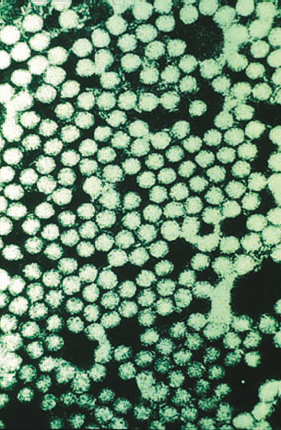
\includegraphics[width=1.1\textwidth]{../FIGS/Electronmicrograph_of_the_foot-and-mouth_disease_virus.png}
  \end{minipage}
  \begin{minipage}{0.65\textwidth}
    \begin{itemize}
      \item Severe, highly communicable \textbf{viral} disease of cattle and swine
      \item Also affects sheep, goats, deer and other cloven-hoofed ruminants. Horses not affected
      \item Elephants, hedgehogs and some rodents also susceptible but do not develop clinical signs of the disease
    \end{itemize}      
  \end{minipage}
\end{frame}

\begin{frame}{}
  \begin{minipage}{0.3\textwidth}
    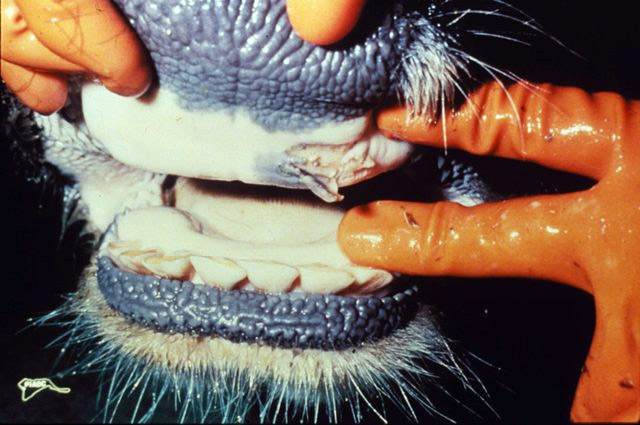
\includegraphics[width=1.1\textwidth]{../FIGS/Foot_and_mouth_disease_in_mouth.jpg}
  \end{minipage}
  \begin{minipage}{0.65\textwidth}
    \begin{itemize}
      \item Fever and blister-like sores on the tongue and lips, in the mouth, on the teats and between the hooves
      \item Many affected animals recover, but the disease leaves them weakened and debilitated
    \end{itemize}
  \end{minipage}
\end{frame}


\begin{frame}{2001 United Kingdom HMD outbreak}
  \begin{itemize}
    \item 2,000 cases of the disease in farms across most of the British countryside
    \vfill
    \item Over 6 million cows and sheep were killed to control the disease
    \vfill
    \item Ministry of Agriculture, Fisheries and Food (MAFF) adopted a policy of ``contiguous cull'' - all sheep within 3,000 metres of known cases slaughtered
  \end{itemize}
\end{frame}

%\maxFrameImage{../FIGS/JamesRushton-FMD-economics-cover-inverted.png}


%%%%%%%%%%%%%%%%%%%
%%%%%%%%%%%%%%%%%%%
\subsection{Symptoms}

\maxFrameImage{../FIGS/Davies-FMD-cover-inverted.png}
\maxFrameImage{../FIGS/Davies-FMD-characteristics-inverted.png}
\maxFrameImage{../FIGS/Davies-FMD-hosts-inverted.png}

\maxFrameImage{../FIGS/Alexandersen_etal-pathogenesis-cover-inverted.png}
\maxFrameImage{../FIGS/Alexandersen_etal-pathogenesis-cows-noBG.png}
\maxFrameImage{../FIGS/Alexandersen_etal-pathogenesis-pigs-noBG.png}



%%%%%%%%%%%%%%%%%%%
%%%%%%%%%%%%%%%%%%%
\subsection{More about transmission}

\maxFrameImage{../FIGS/JamalBelsham-FMD-cover-inverted.png}
\maxFrameImage{../FIGS/JamalBelsham-FMD-genome-inverted.png}

\maxFrameImage{../FIGS/Davies-FMD-cover-inverted.png}
\maxFrameImage{../FIGS/Davies-FMD-pathogenesis-inverted.png}

\maxFrameImage{../FIGS/Alexandersen_etal-pathogenesis-cover-inverted.png}
\maxFrameImage{../FIGS/Alexandersen_etal-pathogenesis-minimum-dose-inverted.png}
\maxFrameImage{../FIGS/Alexandersen_etal-pathogenesis-infectivity-titre-inverted.png}

\maxFrameImage{../FIGS/Arzt_etal-FMD-viral-pathways-cover-inverted.png}
\maxFrameImage{../FIGS/Arzt_etal-FMD-viral-pathways-detection-inverted.png}



%\maxFrameImage{../FIGS/Rweyemamu_etal-FMD-patterns-cover-inverted.png}

%%%%%%%%%%%%%%%%%%%
%%%%%%%%%%%%%%%%%%%
\subsection{Virus types are spatially located}
\maxFrameImage{../FIGS/JamalBelsham-FMD-cover-inverted.png}
\maxFrameImage{../FIGS/JamalBelsham-FMD-geography-inverted.png}


%%%%%%%%%%%%%%%%%%%
%%%%%%%%%%%%%%%%%%%
\subsection{Other reviews worth taking a look at}
\maxFrameImage{../FIGS/GrubmanBaxt-FMD-cover-inverted.png}
\maxFrameImage{../FIGS/Kitching_etal-FMD-cover-inverted.png}


%%%%%%%%%%%%%%%%%%%
%%%%%%%%%%%%%%%%%%%
%%%%%%%%%%%%%%%%%%%
%%%%%%%%%%%%%%%%%%%
\section{A few models}

\maxFrameImage{../FIGS/Keeling-FMD-models-cover-inverted.png}
\maxFrameImage{../FIGS/ThornleyFrance-modelling-FMD-cover-inverted.png}
\maxFrameImage{../FIGS/Ster-FMD-within-farm-cover-inverted.png}
\maxFrameImage{../FIGS/RingaBauch-FMD-pair-approx-cover-inverted.png}
\maxFrameImage{../FIGS/Mushayabasa_etal-model-FMD-cover-inverted.png}


%%%%%%%%%%%%%%%%%%%
%%%%%%%%%%%%%%%%%%%
%%%%%%%%%%%%%%%%%%%
%%%%%%%%%%%%%%%%%%%
\section{Conclusion}

\maxFrameImage{../FIGS/Kitching_etal-FMD-abuse-of-models-cover-inverted.png}
\maxFrameImage{../FIGS/Kitching_etal-FMD-abuse-of-models-table-inverted.png}


\begin{frame}{Conclusion}
\end{frame}


\end{document}
